%%%%%%%%%%%%%%%%%%%%%%%%%%%%%%%%%%%%%%%%%
% Beamer Presentation
% LaTeX Template
% Version 1.0 (10/11/12)
%
% This template has been downloaded from:
% http://www.LaTeXTemplates.com
%
% License:
% CC BY-NC-SA 3.0 (http://creativecommons.org/licenses/by-nc-sa/3.0/)
%
%%%%%%%%%%%%%%%%%%%%%%%%%%%%%%%%%%%%%%%%%

%----------------------------------------------------------------------------------------
%	PACKAGES AND THEMES
%----------------------------------------------------------------------------------------

\documentclass{beamer}
\usepackage{hyperref}
\usepackage{url}
\usepackage{ulem}
\usepackage{tikz}
\usepackage{multicol}
\usetikzlibrary{fit,calc,positioning,decorations.pathreplacing,matrix}
\usetikzlibrary{positioning}
\mode<presentation> {

% The Beamer class comes with a number of default slide themes
% which change the colors and layouts of slides. Below this is a list
% of all the themes, uncomment each in turn to see what they look like.

%\usetheme{default}
%\usetheme{AnnArbor}
%\usetheme{Antibes}
%\usetheme{Bergen}
%\usetheme{Berkeley}
%\usetheme{Berlin}
%\usetheme{Boadilla}
%\usetheme{CambridgeUS}
%\usetheme{Copenhagen}
%\usetheme{Darmstadt}
%\usetheme{Dresden}
%\usetheme{Frankfurt}
%\usetheme{Goettingen}
%\usetheme{Hannover}
%\usetheme{Ilmenau}
%\usetheme{JuanLesPins}
%\usetheme{Luebeck}
%\usetheme{Madrid}
%\usetheme{Malmoe}
%\usetheme{Marburg}
%\usetheme{Montpellier}
%\usetheme{PaloAlto}
%\usetheme{Pittsburgh}
\usetheme{Rochester}
%\usetheme{Singapore}
%\usetheme{Szeged}
%\usetheme{Warsaw}

% As well as themes, the Beamer class has a number of color themes
% for any slide theme. Uncomment each of these in turn to see how it
% changes the colors of your current slide theme.

%\usecolortheme{albatross}
%\usecolortheme{beaver}
%\usecolortheme{beetle}
%\usecolortheme{crane}
%\usecolortheme{dolphin}
%\usecolortheme{dove}
%\usecolortheme{fly}
%\usecolortheme{lily}
%\usecolortheme{orchid}
%\usecolortheme{rose}
%\usecolortheme{seagull}
%\usecolortheme{seahorse}
%\usecolortheme{whale}
%\usecolortheme{wolverine}

%\setbeamertemplate{footline} % To remove the footer line in all slides uncomment this line
%\setbeamertemplate{footline}[page number] % To replace the footer line in all slides with a simple slide count uncomment this line

%\setbeamertemplate{navigation symbols}{} % To remove the navigation symbols from the bottom of all slides uncomment this line
}

\usepackage{graphicx} % Allows including images
\usepackage{booktabs} % Allows the use of \toprule, \midrule and \bottomrule in tables

%----------------------------------------------------------------------------------------
%	TITLE PAGE
%----------------------------------------------------------------------------------------

\title[Algos for FMs]{Algorithms Associated with Factorization Machines} % The short title appears at the bottom of every slide, the full title is only on the title page

\author{Yanyu Liang \\
Xin Lu \\
Xupeng Tong} % Your name
\institute[CMU] % Your institution as it will appear on the bottom of every slide, may be shorthand to save space
{
Carnegie Mellon University \\ % Your institution for the title page
\medskip
\textit{\{yanyul,xlu2,xtong\}@andrew.cmu.edu} % Your email address
}
\date{\today} % Date, can be changed to a custom date

\begin{document}

\begin{frame}
\titlepage % Print the title page as the first slide
\end{frame}

\begin{frame}
\begin{multicols}{2}
\frametitle{Overview} % Table of contents slide, comment this block out to remove it
\tableofcontents % Throughout your presentation, if you choose to use \section{} and \subsection{} commands, these will automatically be printed on this slide as an overview of your presentation
\end{multicols}
\end{frame}

%----------------------------------------------------------------------------------------
%	PRESENTATION SLIDES
%----------------------------------------------------------------------------------------

%------------------------------------------------
\section{Our Problem} % Sections can be created in order to organize your presentation into discrete blocks, all sections and subsections are automatically printed in the table of contents as an overview of the talk
%------------------------------------------------
  \subsection{Factorization Machines}
  \begin{frame}
  \frametitle{Factorization Machines}
    \begin{itemize}
      \item Factorization machines \cite{rendle2010factorization} models $y \in \mathbb{R}$ given $x \in \mathbb{R}^p$ using the following expression:
      \begin{align*}
        \hat{y} &= w_0 + w^T x + \sum_{i, j} (V_ix_i)^T(V_jx_j) \\
        &= w_0 + w^T x + x^T V^T V x
      \end{align*}
      , where $V_i$ is $k \times 1$ vector. 
      \item FMs is widely used in recommendation system, since it implicitly regularizes the model complexity by setting a $k$ which is much smaller than $p$.
    \end{itemize}
  \end{frame}

  \subsection{Other Formulation}
  \begin{frame}
  \frametitle{Other Formulation}
    \begin{itemize}
      \item $\sum_{i, j} (V_ix_i)^T(V_jx_j)$ makes FMs nonconvex, and researcher has proposed convex FMs \cite{blondel2015convex} by replacing low rank constraint by trace norm (replace $V^TV$ with $W$).
      \item Also, by replacing one $V$ in $V^T V$ with $U$, \cite{lin2016non} proposed generalized FMs with an online learning algorithm
    \end{itemize}
  \end{frame}

  \subsection{Our Work}
  \begin{frame}
  \frametitle{Our Goal}
    \begin{itemize}
      \item Propose ADMM method to sovle convexFMs with element-wise $l_1$ constraint
      \item Overview optimization algorithm to solve classic FMs problems
    \end{itemize}
  \end{frame}

%------------------------------------------------
\section{ADMM for sparse convexFMs} % A subsection can be created just before a set of slides with a common theme to further break down your presentation into chunks
%------------------------------------------------
\subsection{ConvexFMs with $l_1$ constraint}
\begin{frame}
\frametitle{ConvexFMs with $l_1$ constraint}
\begin{itemize}
  \item $l_1$ penalty is widely used and it is potential helpful in many applications beyond recommendation systems.
  \item Consider the regression problem in convexFMs with $l_1$ penalty:
    \begin{align*}
      \min_{w_0, w, W} & \sum_{i = 1}^n \underbrace{(y_i - w_0 - w^Tx_i - x_i^T W x_i)^2}_{f(w_0, w, W)} \\
      & + \lambda_1 \|W\|_{\text{tr}} + \lambda_2 \|W\|_1 + \lambda_3 \|w\|_2^2
    \end{align*}
\end{itemize}
\end{frame}

\subsection{ADMM Formulation}
\begin{frame}
\frametitle{ADMM Formulation}
\begin{itemize}
  \item By introduing axilluary variable $U$, it can be fit into ADMM framework and the augmented Lagrangian is:
    \begin{align*}
      \mathcal{L}(w_0, w, W) &= f(w_0, w, W) + \lambda_1 \|U\|_{\text{tr}} + \lambda_2 \|W\|_1 + \lambda_3 \|w\|_2^2 \\
      &+ \langle W - U, u \rangle + m\|W - U\|_2^2 
    \end{align*}
  \item Then the ADMM loop is:
    \begin{enumerate}
    \item Update $w_0, w, W$:
    \begin{align*}
        w_0^k, w^k, W^k &= \arg\min_{w0, w, W} f(w_0, w, W) + \lambda_2 \|W\|_1 \\
        &+ \frac{\rho}{2} \|W - U^{k - 1} + u^{k - 1}\|_2^2
    \end{align*}
    \item Update $U$:
    \begin{align*}
        U^k = \arg\min_U \lambda_1 \|U\|_{\text{tr}} + \frac{\rho}{2}\|W^k - U + u^{k-1}\|_2^2
    \end{align*}
    \item Update $u$:
    \begin{align*}
        u^k = u^{k - 1} + W^k - U^k
    \end{align*}
\end{enumerate}
\end{itemize}
\end{frame}

\subsection{ADMM Subproblem}
\begin{frame}
\frametitle{ADMM Subproblem}
\begin{itemize}
  \item The second step can be solve exactly with proximal operator of trace norm.
  \item We explored two approaches to solve the first subprobelm:
    \begin{itemize}
      \item proximal graident descent on $w_0, w, W$ (proximal)
      \item blockwise coordinate descent on $w_0, w$ and $W$ respectively, where we applied coordinate descent on the first block and tried proximal gradient (coor-proximal) and Quasi-Newton (coor-newton) method on the second block
    \end{itemize}
\end{itemize}
\end{frame}

\subsection{ADMM Results}
\begin{frame}
\frametitle{ADMM Results}
\begin{itemize}
  \item Quasi-Newton method performs better than proximal graident descent in solving $\arg\min_W g(W)$ subproblem (as we expected)
  \item proximal gradient descent performs better and stable than blockwise coordinate descent
  \begin{figure}[htbp]
  \centering
  \begin{minipage}{0.45\textwidth}
    \centering
    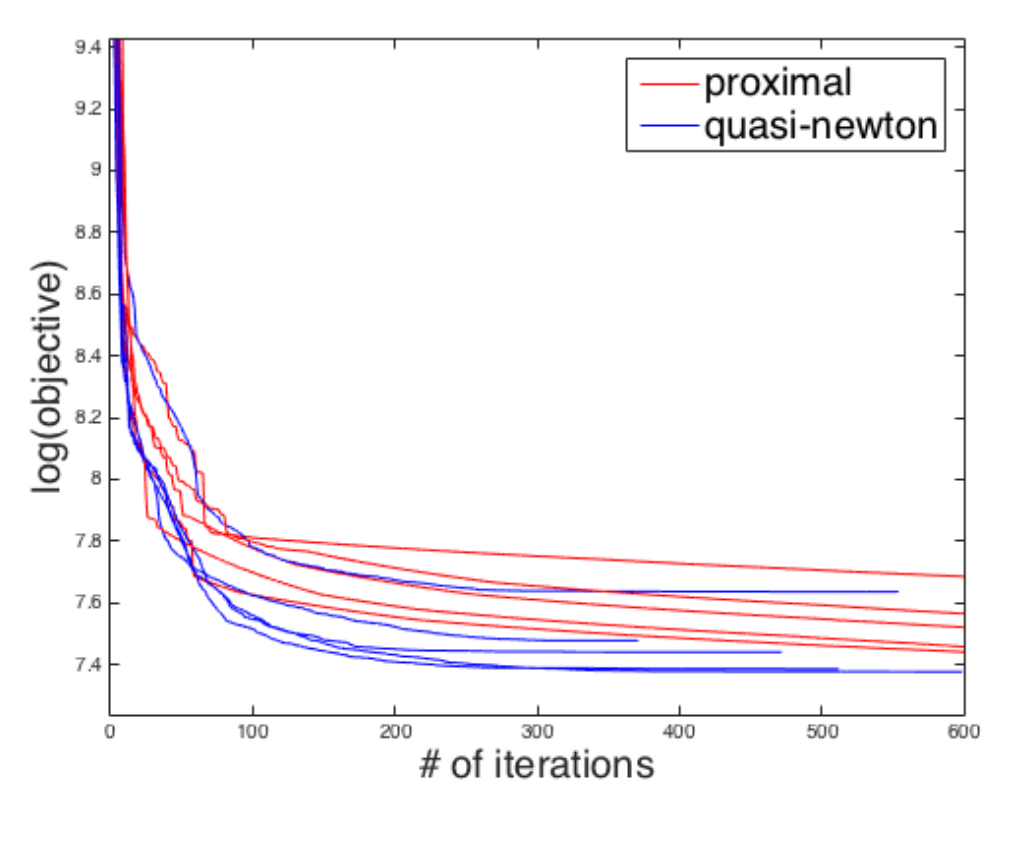
\includegraphics[width=1\textwidth]{images/argminW}
  \end{minipage}
  \hfill
  \begin{minipage}{0.45\textwidth}
    \centering
    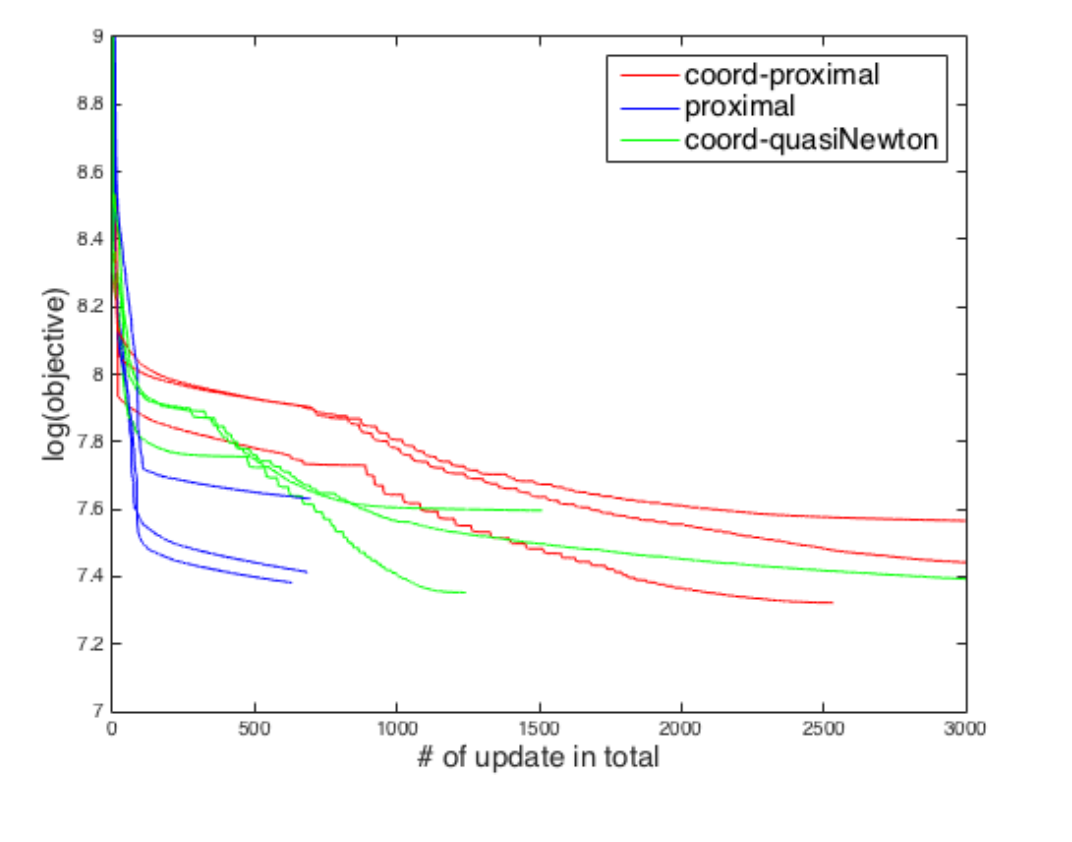
\includegraphics[width=1\textwidth]{images/argminw0wW}
  \end{minipage}
  \end{figure}
\end{itemize}
\end{frame}

\subsection{ADMM Results (con'd)}
\begin{frame}
\frametitle{ADMM Results}
\begin{itemize}
  \item ADMM converges and it achieves feasiblity along the path
  \item with the same number of updates (consider inner loop), ADMM outperforms sub-gradient method
  \begin{figure}[htbp]
  \centering
  \begin{minipage}{0.35\textwidth}
    \centering
    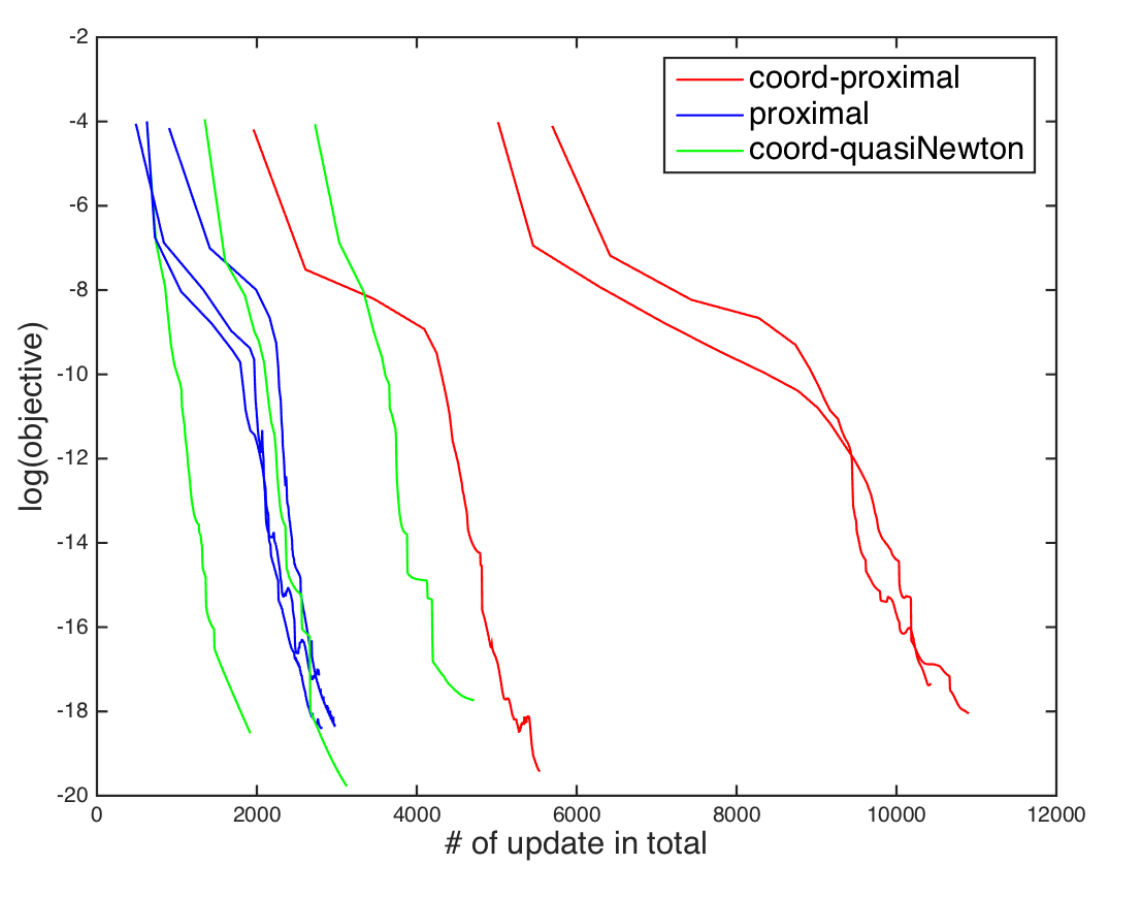
\includegraphics[width=1\textwidth]{images/feasibility}
  \end{minipage}
  \hfill
  \begin{minipage}{0.35\textwidth}
    \centering
    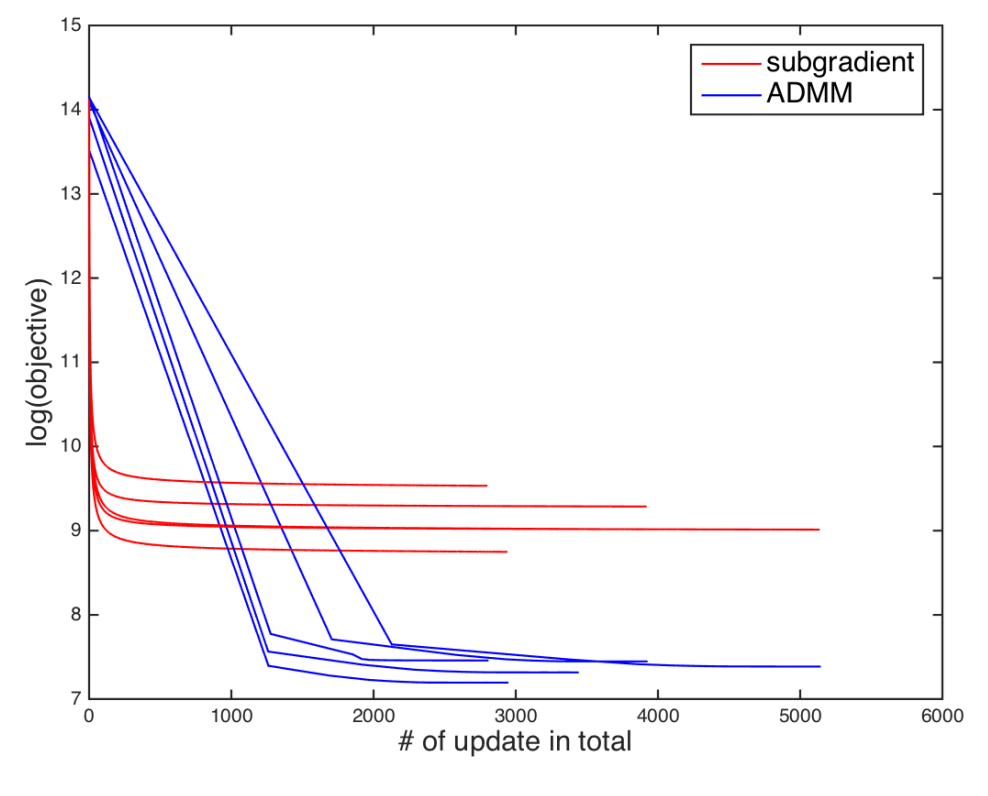
\includegraphics[width=1\textwidth]{images/subgrad}
  \end{minipage}
  \end{figure}
\end{itemize}
\end{frame}



%------------------------------------------------
\begin{frame}[allowframebreaks]
\frametitle{References}
\footnotesize
\bibliography{mybib} 
\bibliographystyle{IEEEtran}
\end{frame}

%------------------------------------------------

\begin{frame}
\Huge{\centerline{The End}}
\end{frame}

%----------------------------------------------------------------------------------------

\end{document} 